% SAHARA capstone project report, MPSTME format (Capstone guidelines 2026-27, Annexure A.8).
% Build: tectonic -X compile sahara_report.tex
\documentclass[12pt,a4paper,oneside]{report}
\usepackage{fontspec}
\setmainfont{Times New Roman}
\usepackage[left=1.5in,right=1in,top=1in,bottom=1in,headheight=15pt]{geometry}
\usepackage{setspace}
\onehalfspacing
\usepackage{graphicx,xcolor,booktabs,array,longtable,tabularx,enumitem,amsmath,amssymb}
\usepackage{tikz}
\usetikzlibrary{arrows.meta,positioning,shapes.geometric,calc}
\usepackage{fancyhdr}
\usepackage{titlesec}
\usepackage[font=small,labelfont=bf]{caption}
\usepackage[hidelinks]{hyperref}
\usepackage{url}
\graphicspath{{../assets/}}
\renewcommand{\bibname}{References}

% Captions: Times New Roman 10; figure names below, table names above.
\captionsetup{font={footnotesize}, labelfont=bf}
\captionsetup[table]{position=above}

% Chapter 18 bold, section 14 bold, subsection 12 bold.
\titleformat{\chapter}[display]{\centering\fontsize{18}{22}\selectfont\bfseries}{Chapter \thechapter}{6pt}{}
\titlespacing*{\chapter}{0pt}{0pt}{18pt}
\titleformat{\section}{\fontsize{14}{17}\selectfont\bfseries}{\thesection}{0.6em}{}
\titleformat{\subsection}{\fontsize{12}{15}\selectfont\bfseries}{\thesubsection}{0.6em}{}

% Header: project title (left), academic year (right); footer: page number (right).
\newcommand{\shorttitle}{SAHARA: On-Device Sound Alerts for DHH Users}
\pagestyle{fancy}
\fancyhf{}
\fancyhead[L]{\small\shorttitle}
\fancyhead[R]{\small A.Y. 2026--2027}
\fancyfoot[R]{\thepage}
\fancypagestyle{plain}{\fancyhf{}\fancyhead[L]{\small\shorttitle}\fancyhead[R]{\small A.Y. 2026--2027}\fancyfoot[R]{\thepage}}

\newcommand{\ptitle}{SAHARA: A Real-Time, On-Device Sound Event Detection and Dual-Channel Alert System for the Deaf and Hard-of-Hearing, with India-Specific Acoustic Adaptation}
\renewcommand{\arraystretch}{1.15}

\begin{document}

% ---------------------------------------------------------------- Title page
\begin{titlepage}
\thispagestyle{empty}
\centering
{\fontsize{18}{24}\selectfont\bfseries \ptitle\par}
\vspace{0.8cm}
{\large Project Report submitted in the partial fulfilment\\ of\\[2mm] \textbf{Bachelor of Technology}\\ in\\[2mm] \textbf{Computer Engineering}\\[4mm] by\par}
\vspace{4mm}
{\large
\begin{tabular}{lll}
Raj Singh & (B125) & 70022300051\\
Prachi Teotia & (B132) & 70022300162\\
Advika Mishra & (B076) & 70022300146\\
Mahi Mayani & (B073) & 70022300180\\
\end{tabular}\par}
\vspace{6mm}
{\large Under the supervision of\\[2mm] \textbf{Prof.\ Priti Rumao}\\ (Department of Computer Engineering, MPSTME)\par}
\vfill

\includegraphics[width=0.45\textwidth]{mpstme_logo.png}\\[2mm]
{\large SVKM's NMIMS University\\ (Deemed-to-be University)\\ \textbf{MUKESH PATEL SCHOOL OF TECHNOLOGY MANAGEMENT \& ENGINEERING (MPSTME)}\\ Vile Parle (W), Mumbai-56\\[2mm] A.Y. 2026--2027\par}
\end{titlepage}

\pagenumbering{roman}
\setcounter{page}{2}

% ---------------------------------------------------------------- Certificate
\chapter*{Certificate}
\addcontentsline{toc}{chapter}{Certificate}
\begin{center}
SVKM's NMIMS University (Deemed-to-be University)\\
MUKESH PATEL SCHOOL OF TECHNOLOGY MANAGEMENT \& ENGINEERING (MPSTME)\\
Vile Parle (W), Mumbai-56\\
(A.Y. 2026--2027)
\end{center}
\vspace{6mm}
This is to certify that the project entitled ``\ptitle'' has been done by Mr.\ Raj Singh, Ms.\ Prachi Teotia, Ms.\ Advika Mishra and Ms.\ Mahi Mayani under my guidance and supervision and has been submitted in partial fulfilment of the degree of Bachelor of Technology in Computer Engineering of MPSTME, SVKM's NMIMS (Deemed-to-be University), Mumbai, India.

\vspace{2.5cm}
\noindent\begin{tabular}{@{}p{0.45\textwidth}p{0.45\textwidth}@{}}
\rule{5.5cm}{0.4pt} & \rule{5.5cm}{0.4pt}\\
Project Mentor (Internal Guide) & Examiner\\
Prof.\ Priti Rumao & (Name and Signature)\\
Date: & \\
\end{tabular}

\vspace{2cm}
\noindent Place: Mumbai \hfill
\begin{tabular}[t]{@{}l@{}}\rule{5.5cm}{0.4pt}\\ (HoD) (Name and Signature)\end{tabular}

% ---------------------------------------------------------------- Acknowledgement
\chapter*{Acknowledgement}
\addcontentsline{toc}{chapter}{Acknowledgement}
We express our sincere gratitude to our mentor, Prof.\ Priti Rumao, for her guidance, encouragement and constructive feedback throughout this capstone project. We thank the Head of the Department and the faculty of the Department of Computer Engineering, MPSTME, for their support and for the facilities provided, and the capstone project committee for the reviews that shaped this work. We are grateful to our families and friends who helped us record sounds in their homes, and to the reviewers of ICEI 2026, whose comments improved our research paper. We also acknowledge the creators of the open datasets and models on which this work builds: AudioSet, FSD50K, ESC-50, DESED, YAMNet and openWakeWord.

\vspace{1cm}
\begin{center}
\begin{tabular}{lll}
\toprule
\textbf{Name} & \textbf{Roll No.} & \textbf{SAP ID}\\
\midrule
Raj Singh & B125 & 70022300051\\
Prachi Teotia & B132 & 70022300162\\
Advika Mishra & B076 & 70022300146\\
Mahi Mayani & B073 & 70022300180\\
\bottomrule
\end{tabular}
\end{center}

% ---------------------------------------------------------------- Abstract
\chapter*{Abstract}
\addcontentsline{toc}{chapter}{Abstract}
People who are Deaf or Hard-of-Hearing (DHH) cannot rely on sound to notice a smoke alarm, a siren, a doorbell, a crying baby or someone calling their name. Existing sound-awareness tools are rarely evaluated on how often they alert falsely, often depend on the cloud or on a smartwatch, and are seldom tested in Indian homes, whose doorbells, appliances and street sounds differ from the Western recordings that dominate public datasets.

This project presents SAHARA, a real-time sound event detection and alert system that runs entirely on an Android phone. A native foreground service keeps the last second of audio in memory, a frozen YAMNet network turns it into a 1,024-dimensional embedding every half second, and a small trained classifier head (296,328 parameters) scores eight household sounds: smoke alarm, siren, glass break, doorbell, knocking, dog bark, baby cry and appliance beep. Instead of a fixed threshold, each class's threshold and the number of recent windows that must exceed it are tuned jointly on validation data against an explicit budget of four false alarms per hour, with missed safety sounds weighted three times. A separate speech path tells the user when their name is called and, for enrolled family members, by whom. Every alert is shown full-screen and played as a class-coded vibration pattern on the phone; the same patterns are implemented in the firmware of a proposed ESP32 Bluetooth wristband costing about Rs.~870. No audio is ever stored and the release application has no Internet permission.

The model was trained on 22,549 clips from FSD50K, AudioSet, ESC-50 and DESED and on SAHARA-IN, 329 clips recorded by the team in Mumbai homes and streets. On held-out public data it reaches 0.778 mean average precision and raises 3.5 false alarms per hour of continuous background audio; on the same model, budget tuning reduces false alarms from 34.1 to 6.1 per hour. Cross-validation on SAHARA-IN shows that the Indian recordings raise mean average precision from 0.621 to 0.822 for homes the model has heard, but not for unseen recording sessions (0.600); a three-recording home calibration step therefore raises the share of events alerted in unseen homes from 19\,\% to 35\,\%. On a Samsung Galaxy S24, inference takes 20--29\,ms per window. A research paper describing the work has been submitted to ICEI 2026.

\tableofcontents
\addcontentsline{toc}{chapter}{List of Figures}
\listoffigures
\addcontentsline{toc}{chapter}{List of Tables}
\listoftables

\chapter*{Abbreviations}
\addcontentsline{toc}{chapter}{Abbreviations}
\begin{longtable}{@{}p{3cm}p{10.5cm}@{}}
\toprule
\textbf{Abbreviation} & \textbf{Full form}\\
\midrule
\endhead
AP & Average Precision\\
AUC & Area Under the (ROC) Curve\\
BLE & Bluetooth Low Energy\\
BOM & Bill of Materials\\
CV & Cross-Validation\\
DESED & Domestic Environment Sound Event Detection dataset\\
DHH & Deaf and Hard-of-Hearing\\
EER & Equal Error Rate\\
ESC-50 & Environmental Sound Classification dataset (50 classes)\\
FA/h & False alarms per hour\\
FSD50K & Freesound Dataset 50k\\
GATT & Generic Attribute Profile (Bluetooth)\\
GE2E & Generalised End-to-End (speaker verification loss)\\
mAP & mean Average Precision\\
MOSFET & Metal-Oxide-Semiconductor Field-Effect Transistor\\
PCM & Pulse-Code Modulation\\
ROC & Receiver Operating Characteristic\\
SAHARA & Sound-based Alert and Haptic Assistance for Real-time Awareness\\
SAHARA-IN & SAHARA's Indian field recording set\\
SNR & Signal-to-Noise Ratio\\
TFLite & TensorFlow Lite\\
VAD & Voice (energy) Activity Detection\\
YAMNet & Yet Another Mobile Network (audio event classifier)\\
\bottomrule
\end{longtable}

% ================================================================ Chapter 1
\clearpage
\pagenumbering{arabic}
\chapter{Introduction}
This chapter introduces the problem SAHARA addresses, the motivation and scope of the work, the problem statement, the main contributions and the organisation of the report.

\section{Background of the Project Topic}
More than 1.5 billion people live with some degree of hearing loss, and over 430 million with disabling loss \cite{who2021}. In India an estimated 63 million people have significant auditory impairment \cite{nppcd}, and the 2011 Census recorded over five million people with a hearing disability \cite{census2011}. For these people everyday sounds that carry safety or social information are inaudible: a smoke alarm or an approaching siren signals danger, a doorbell or knock signals a visitor, a microwave beep signals that food is ready, a crying baby needs attention, and a family member calling their name needs them. Unless such sounds are converted into a visual or tactile signal, the information is simply lost.

Machine learning has made automatic sound recognition practical. Large labelled collections such as AudioSet \cite{gemmeke2017} and FSD50K \cite{fonseca2022} allow deep networks to learn general-purpose audio representations \cite{hershey2017,kong2020}, and compact models such as YAMNet \cite{yamnet}, built on MobileNet \cite{howard2017}, run in real time on mobile phones. Research systems for DHH users have used these advances on phones, smart displays and smartwatches \cite{bragg2016,jain2020homesound,jain2020soundwatch,jain2022protosound}.

\section{Motivation and Scope of the Report}
Three gaps motivated this project. First, sound-awareness systems are usually evaluated with symmetric, threshold-free metrics such as accuracy, while what a user lives with is a stream of alerts: a missed fire alarm can be fatal, and frequent false alarms lead users to ignore or switch off the aid \cite{jain2020homesound,huang2023}. Second, many systems send audio or features to a server, which is unacceptable for a device that listens continuously inside a home. Third, public datasets come mostly from Western environments; Indian homes add pressure-cooker whistles, temple bells, street hawkers and monsoon rain, and Indian doorbells are often melodic chimes.

The scope of this report is the complete SAHARA system: data collection and curation, the on-device model and alert policy, the Android application, the name-call and caller-identification path, the evaluation on public and Indian data, and the design of a low-cost haptic wristband. The wristband's firmware and Bluetooth protocol are implemented; building and measuring the hardware is future work.

\section{Problem Statement}
To design and implement a real-time sound event detection and alert system for DHH users that (a) detects eight safety-critical and everyday household sounds on a mobile phone without any network connection or stored audio, (b) keeps false alarms to a stated budget while prioritising safety-critical sounds, (c) is evaluated on recordings from Indian homes, (d) tells the user when their name is called and by whom, and (e) delivers alerts as distinguishable vibration patterns on the phone and on an affordable wearable.

\section{Salient Contributions}
\begin{enumerate}[itemsep=2pt]
\item \textbf{Alerting tuned to a false-alarm budget}: per-class thresholds and temporal rules chosen jointly to maximise safety-weighted detection subject to four false alarms per hour; on the same model this cuts false alarms on test audio from 34.1 to 6.1 per hour.
\item \textbf{Privacy by construction}: all inference runs on the phone; audio exists only in a one-second memory buffer and the release application has no Internet permission.
\item \textbf{Name calls for any voice}, with enrolled callers named (``Raj is calling you'') and others reported as ``Someone''.
\item \textbf{SAHARA-IN}, 329 sound clips and 107 name-call clips recorded in Mumbai, evaluated with both random and session-held-out cross-validation, and a \textbf{home calibration} step that adapts thresholds to a household from three recordings.
\item \textbf{A wristband design}: Bluetooth protocol, ESP32 firmware with nine class-coded vibration patterns shared with the phone, and a bill of materials of about Rs.~870.
\end{enumerate}

\section{Organisation of the Report}
Chapter 2 reviews related work and identifies the research gap. Chapter 3 describes the methodology and implementation: system architecture, hardware, software, data and training. Chapter 4 presents and analyses the results. Chapter 5 lists advantages, limitations and applications, and Chapter 6 concludes with the scope for future work. Appendices give flowcharts, data sheets, the list of components and the paper submitted.

\textit{Summary:} SAHARA targets a real safety gap for DHH users and is designed around three requirements that prior systems leave open: measured false alarms, privacy and Indian conditions.

% ================================================================ Chapter 2
\chapter{Literature Survey}
This chapter reviews research on sound awareness for DHH users, audio representation learning, sound event detection datasets and metrics, keyword spotting and speaker recognition, and wearable delivery, and ends with the research gap that defines our problem.

\section{Introduction to the Overall Topic}
Sound event detection identifies which sound events occur in an audio stream and when \cite{mesaros2021}. Modern systems learn from large labelled corpora: AudioSet provides over two million ten-second YouTube clips labelled with a 527-class ontology \cite{gemmeke2017}, FSD50K provides 51,197 human-verified Freesound clips \cite{fonseca2022}, ESC-50 provides 2,000 curated environmental clips in 50 classes \cite{piczak2015}, and DESED provides domestic soundscapes for detection in homes \cite{turpault2019}. Convolutional networks trained on such data give transferable embeddings: VGGish \cite{hershey2017}, OpenL3 \cite{cramer2019}, PANNs \cite{kong2020}, the Audio Spectrogram Transformer \cite{gong2021} and YAMNet \cite{yamnet}, a MobileNetV1 \cite{howard2017} trained on AudioSet. Data augmentation \cite{salamon2017} and learning from weak, clip-level labels \cite{kumar2016} make small task-specific sets usable. Evaluation of polyphonic detection is itself a research topic \cite{mesaros2016}, and the asymmetric cost of errors is studied in cost-sensitive learning \cite{elkan2001}. Quantisation and mobile runtimes \cite{jacob2018} make continuous inference feasible on phones. Applying these tools to assistive technology for DHH users raises questions of what to detect, how to notify and how to keep false alarms low \cite{matthews2006,bragg2016,findlater2019,goodman2020}. The World Health Organization's World Report on Hearing frames the scale of the need \cite{who2021}.

\section{Survey of Related Work}
\textbf{Visualising non-speech sound.} Matthews et al. \cite{matthews2006} studied how DHH people want non-speech sounds presented, finding that awareness of sounds such as alarms, doorbells and people approaching matters at home and at work, and that visualisations must be glanceable. This established the need for automatic sound awareness, but the systems of the time relied on simple energy cues rather than recognition.

\textbf{Personalisable mobile detection.} Bragg et al. \cite{bragg2016} designed a personalisable mobile sound detector and showed in a study with DHH participants that users want to choose which sounds they are alerted to and to teach the system household-specific sounds. The work demonstrated feasibility on a phone but did not report false alarms over continuous audio.

\textbf{Preferences for wearable delivery.} Findlater et al. \cite{findlater2019} surveyed 201 DHH participants and found strong interest in sound awareness delivered through wearable and mobile devices, with haptic and visual feedback, and a desire to prioritise urgent sounds. Goodman et al. \cite{goodman2020} then evaluated smartwatch-based sound feedback across contexts and found that usefulness depends strongly on the situation and on alert accuracy. Mielke and Br\"uck \cite{mielke2015} piloted a smartwatch as an assistive device for deaf people. These studies motivated SAHARA's vibration patterns and wristband.

\textbf{In-home deployment.} Jain et al. \cite{jain2020homesound} deployed HomeSound, an in-home sound awareness system with displays in several rooms, in DHH households over weeks. Participants valued the awareness, but false and missed alerts quickly eroded trust. This finding is the direct motivation for SAHARA's false-alarm budget.

\textbf{Smartwatch recognition.} SoundWatch \cite{jain2020soundwatch} compared deep learning architectures for smartwatch-based sound recognition and analysed the trade-offs between accuracy, latency and battery life on watch and phone. It showed that real-time recognition on wearables is practical, but required users to own a compatible smartwatch and reported clip-level accuracy rather than alert rates.

\textbf{Location-independent sound awareness.} UbiEar \cite{liu2017ubiear} brought sound awareness to hard-of-hearing users on smartphones in any location, addressing the variability of real acoustic environments, again with clip-level evaluation.

\textbf{Plug-and-play activity recognition.} Ubicoustics \cite{laput2018} showed that models trained on professional sound-effect libraries transfer to real-world acoustic activity recognition with little or no in-situ data, supporting SAHARA's choice of a pretrained embedding with a small trained head.

\textbf{Few-shot personalisation.} ProtoSound \cite{jain2022protosound} used prototypical networks \cite{snell2017} so that DHH users can add personal sounds from a few examples, and Goodman et al. \cite{goodman2021} studied how users themselves train sound recognisers. SAHARA's custom sounds and home calibration follow this line.

\textbf{Field feasibility.} Huang et al. \cite{huang2023} ran a three-week field study of mobile sound recognition with DHH participants and concluded that the technology is ``not there yet'': background noise, sound variability and confusable classes cause errors that users notice. This supports SAHARA's focus on measured false alarms and on adapting to each home.

\textbf{Keyword spotting and speaker recognition.} Lin et al. \cite{lin2020} showed that speech embeddings pretrained for keyword spotting allow a small head to learn a new word from limited and synthesised data, as packaged by openWakeWord \cite{openwakeword}. Wan et al. \cite{wan2018} introduced the GE2E loss for compact speaker embeddings used in verification. SAHARA combines both to detect a user's name and identify enrolled callers.

\textbf{Alarm signal standards.} ISO 8201 \cite{iso8201} specifies the ``temporal-three'' evacuation signal of fire alarms; SAHARA uses the same rhythm for its smoke-alarm vibration so that the pattern matches what users may already know.

Table~\ref{tab:litcomp} compares the closest systems.

\begin{table}[h]
\caption{Comparison of related sound-awareness systems with SAHARA}
\label{tab:litcomp}
\centering\small
\begin{tabularx}{\textwidth}{@{}lXccc@{}}
\toprule
System & Platform and key finding & On-device & FA/h reported & Indian data\\
\midrule
Bragg et al. 2016 \cite{bragg2016} & Phone app; users want personalisation & Yes & No & No\\
HomeSound 2020 \cite{jain2020homesound} & Home displays; false alerts erode trust & Partly & No & No\\
SoundWatch 2020 \cite{jain2020soundwatch} & Smartwatch; accuracy vs.\ battery & Yes & No & No\\
UbiEar 2017 \cite{liu2017ubiear} & Smartphone; location independence & Yes & No & No\\
ProtoSound 2022 \cite{jain2022protosound} & Phone; few-shot personal sounds & Yes & No & No\\
Huang et al. 2023 \cite{huang2023} & Field study; noise and confusions & Yes & No & No\\
\textbf{SAHARA} & Phone + wristband design; budget-tuned alerts, name calls & Yes & Yes & Yes\\
\bottomrule
\end{tabularx}
\end{table}

\section{Research Gap}
The survey shows that (i) none of the systems tunes its alert rule to an explicit false-alarm rate or reports false alarms per hour of continuous audio, although false alarms are the main reason users lose trust; (ii) none is evaluated on recordings from Indian homes; (iii) most assume the user owns a commercial smartwatch for haptic delivery; and (iv) name calls, one of the most socially important sounds, are not handled for arbitrary voices with caller identification. SAHARA's problem statement (Section 1.3) addresses these four gaps.

\textit{Summary:} prior work establishes that DHH users want accurate, glanceable, wearable sound awareness and that false alerts erode trust; the missing pieces are budgeted alerting, Indian evaluation, low-cost delivery and name calls.

% ================================================================ Chapter 3
\chapter{Methodology and Implementation}
This chapter describes the block diagram of the system, the hardware, the software (Android application, model and alert policy), the data pipeline and the training and tuning methods.

\section{Block Diagram}
Fig.~\ref{fig:arch} shows the complete pipeline. Everything runs on the phone inside an Android foreground service; only a class identifier and an intensity byte cross the Bluetooth link to the wristband.

\begin{figure}[h]
\centering
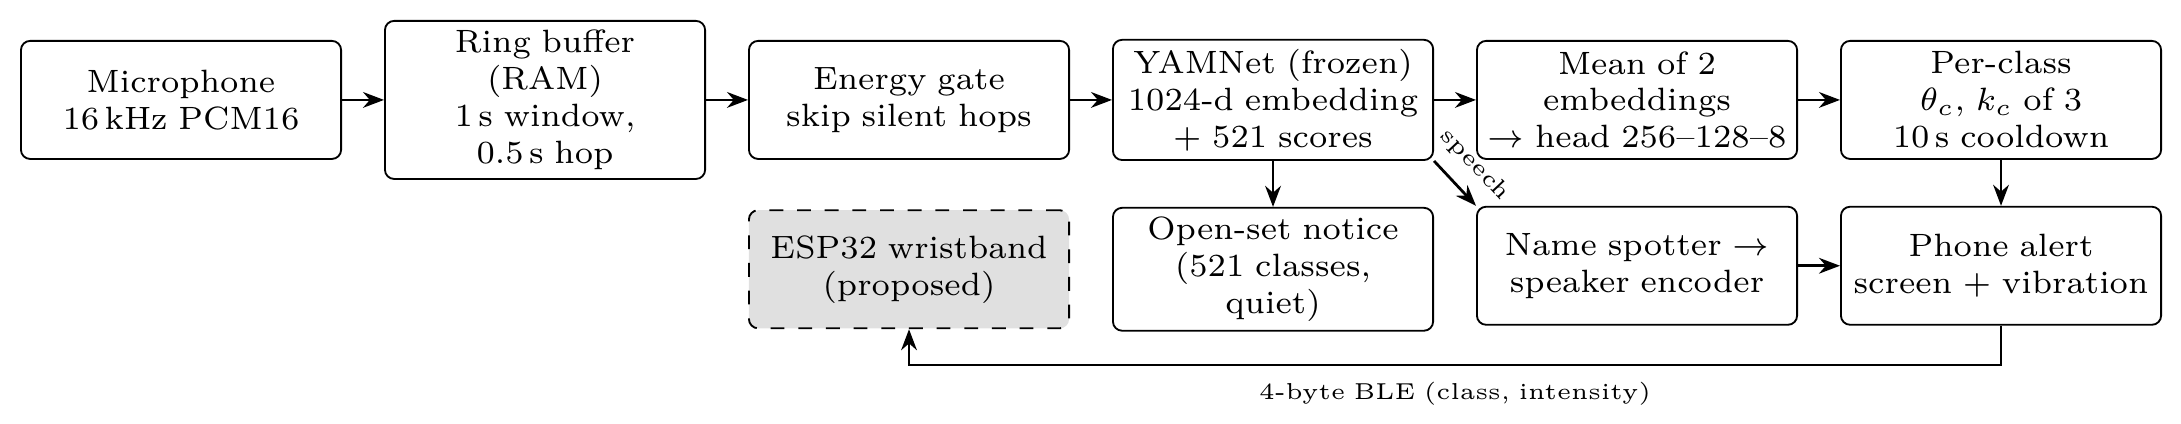
\includegraphics[width=\textwidth]{architecture.png}
\caption{SAHARA block diagram: on-phone processing from microphone to alert, and the proposed wristband (dashed)}
\label{fig:arch}
\end{figure}

\section{Hardware Description}
\textbf{Phone.} SAHARA was developed and measured on a Samsung Galaxy S24 (Android 16); the application supports Android 8.0 (API 26) and above. The built-in microphone is read at 16\,kHz, 16-bit mono.

\textbf{Wristband (designed).} The wristband is an ESP32-WROOM-32 Bluetooth Low Energy peripheral (Appendix B) with a 10\,mm coin vibration motor driven through an AO3400 logic-level MOSFET with 20\,kHz PWM, a 500\,mAh LiPo cell, a protected TP4056 USB-C charger and a low-dropout 3.3\,V regulator; a resistor divider lets the board read its battery voltage. The motor runs from the cell through the MOSFET so that its current never sags the 3.3\,V rail. The bill of materials totals about Rs.~870 (Appendix C). The firmware clocks the CPU at 80\,MHz, transmits at $+3$\,dBm and requests a 30--50\,ms connection interval, targeting an alert delivery delay below about 150\,ms. Below 20\,\% charge it lowers motor strength and transmit power, and at 3.4\,V it enters deep sleep. When the phone disconnects, two long buzzes tell the user that alerts have stopped. From datasheet currents we estimate 30--50\,mA while connected on the development board, or about 10--15 hours on the cell; these figures must be measured on the built device.

\begin{table}[h]
\caption{Wristband alert protocol (Bluetooth GATT, 4 bytes, phone to band)}
\label{tab:ble}
\centering\small
\begin{tabular}{@{}clp{8cm}@{}}
\toprule
Byte & Field & Values\\
\midrule
0 & version & \texttt{0x01}\\
1 & command & \texttt{0x01} alert, \texttt{0x02} test, \texttt{0x03} stop\\
2 & class id & 0--7 sound classes; \texttt{0x20} name call\\
3 & intensity & 255 for safety classes, otherwise confidence $\times$255 (at least 128)\\
\bottomrule
\end{tabular}
\end{table}

\section{Software Description}
\subsection{Android Application}
The application is written in Flutter (user interface) with a native Kotlin module (audio capture, inference and alerts). A foreground service keeps listening with the screen off and after the app is swiped away. Samples enter a one-second ring buffer that advances every 0.5\,s; a mean-square energy gate ($10^{-4}$) skips silent hops to save battery. Each remaining 0.975\,s patch is embedded by YAMNet (TensorFlow Lite) into a 1,024-dimensional vector, and the same pass yields YAMNet's 521 AudioSet class scores. The mean of the two latest non-silent embeddings feeds the classifier head (Dense 256, ReLU, dropout; Dense 128, ReLU, dropout; Dense 8, sigmoid; 296,328 parameters). The training code computes exactly the same window vectors as the phone, and a test asserts a maximum difference of 0.0.

The user interface shows a full-screen alert with the sound's name and time, keeps a history of alerts (label, confidence and time only), and offers settings for which sounds to alert on, a five-step sensitivity, vibration, enrolment of callers, custom sounds and home calibration.

\textbf{Privacy.} Audio exists only in the ring buffer and is overwritten every 0.5\,s. Nothing is written to storage, the release build declares no Internet permission, and enrolment for callers, custom sounds and calibration keeps only numbers (embeddings or thresholds), never audio. On the Galaxy S24 we confirmed that app storage holds no audio files after listening.

\subsection{Name Calls and Caller Identification}
When YAMNet's speech score is at least 0.2, pretrained speech embeddings \cite{lin2020,openwakeword} turn the last two seconds into a sequence of 96-dimensional vectors every 80\,ms, and a standardised logistic regression over eight consecutive vectors detects the user's name (``Aryan''). The head was trained on 38 recordings of the name by four team members, each also mixed with Indian background at 5--20\,dB, against similar names (Arya, Aryanshi and others) and background scenes. When it fires, a GE2E speaker encoder \cite{wan2018} (three-layer LSTM, reimplemented in Kotlin) embeds the same audio into 256 numbers and compares it by cosine similarity with each enrolled caller's mean embedding: at 0.70 or more the alert reads ``Raj is calling you'', otherwise ``Someone is calling you''. Naming the wrong person is worse than ``Someone'', because with ``Someone'' the user still learns that they are being called.

\subsection{Open-Set Notices and Custom Sounds}
Sounds outside the eight classes that YAMNet recognises with score of at least 0.35 in two of three windows (for example a tap running or a cat) produce a quiet notification without vibration, with a 30\,s cooldown; they are suppressed while a trained class fires, so they never compete with safety alerts. Users can also enrol a household sound from five to ten three-second recordings; its prototype is the mean of centred, normalised YAMNet window vectors, matched by cosine similarity, in the spirit of ProtoSound \cite{jain2022protosound}.

\subsection{Class-Coded Haptics}
Each sound has a distinct vibration rhythm (Fig.~\ref{fig:haptics}), played identically by the phone (with amplitude control) and by the wristband firmware; an automated test fails the build if the two copies differ. The smoke alarm uses the temporal-three rhythm of evacuation alarms \cite{iso8201}, a siren is a rising and falling swell, a doorbell a strong-then-soft ``ding-dong'', knocking four quick taps, and a name call two medium and two short buzzes.

\begin{figure}[h]
\centering
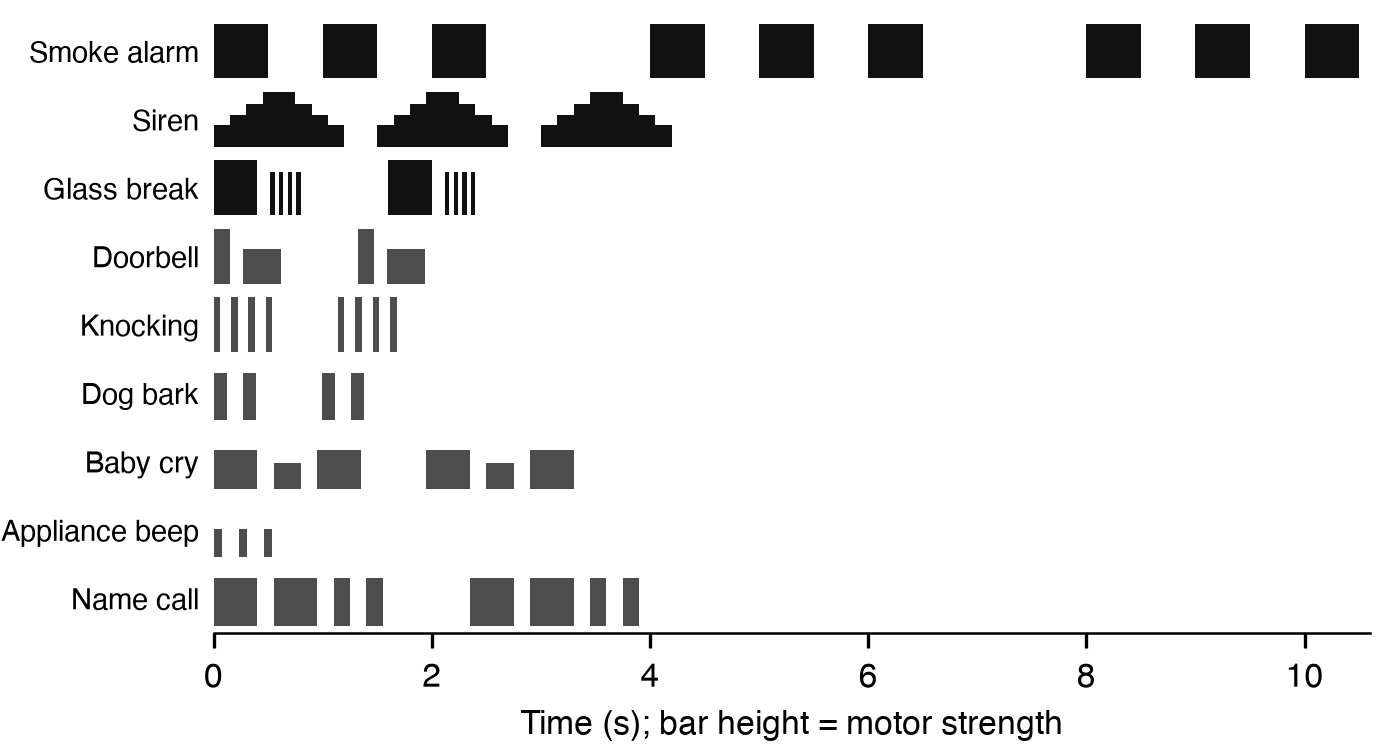
\includegraphics[width=0.85\textwidth]{haptics.png}
\caption{Vibration patterns of the nine alert types on one time scale; bar height is motor strength}
\label{fig:haptics}
\end{figure}

\section{Data Pipeline}
\subsection{Public Data}
Target clips come from FSD50K, AudioSet and ESC-50; background comes from 10,000 FSD50K clips without any target-like label, the 44 non-target ESC-50 categories and DESED real soundscapes (Table~\ref{tab:data}). Every label identifier was verified against the official vocabularies. This removed serious errors in an earlier build: four AudioSet identifiers pointed to the wrong classes, 64 of 188 AudioSet clips did not carry their class's label, and FSD50K's generic \textit{Alarm} (mostly telephones and car alarms) had been mapped to appliance beep. Every class now has at least 150 real clips and at least 20 in the test split. Splits are 70/15/15, grouped by upstream recording, so that the same recording never appears in training in one dataset and in test in another.

\begin{table}[h]
\caption{Real clips per class and source (test clips in brackets); $^\dagger$ marks safety-critical classes. Background also includes 605 DESED clips}
\label{tab:data}
\centering\small
\begin{tabular}{@{}lrrrrr@{}}
\toprule
Class & AudioSet & ESC-50 & FSD50K & SAHARA-IN & Total (test)\\
\midrule
Smoke alarm$^\dagger$ & 183 & -- & -- & 20 & 203 (35)\\
Doorbell & 92 & -- & 144 & 58 & 294 (57)\\
Siren$^\dagger$ & 34 & 40 & 132 & 20 & 226 (42)\\
Knocking & 97 & 40 & 373 & 67 & 577 (100)\\
Dog bark & 10 & 40 & 536 & 11 & 597 (94)\\
Baby cry & 106 & 40 & -- & 14 & 160 (30)\\
Glass break$^\dagger$ & 97 & 40 & 510 & 20 & 667 (105)\\
Appliance beep & 261 & 40 & 206 & 59 & 566 (101)\\
Background & -- & 1,760 & 10,000 & 60 & 12,425 (1,876)\\
\bottomrule
\end{tabular}
\end{table}

\subsection{SAHARA-IN Field Recordings}
The four team members recorded 329 clips on their own phones in Mumbai homes and streets, in three uploads: 269 target clips (67 knocking, 59 appliance beep, 58 doorbell, 20 each of smoke alarm, siren and glass break, 14 baby cry and 11 dog bark) and 60 background clips (street hawkers, a temple, a kitchen, television, monsoon rain, and hard negatives such as drawers, doors and a washing machine spinning without beeping). Because every recording was made under different conditions, the split is by label rather than by recorder: about 40\,\% of each label, spread across its recording conditions, is held out for test, and each upload is split on its own so that adding clips never moves an earlier one. A further 107 clips (38 of the name ``Aryan'' and 69 of similar names) serve the name-call model. Because the recordings come from a few sittings, each clip's recording session is inferred (its recorder, or for unattributed uploads the phone's numbered file-name series) so that cross-validation can also hold out whole sessions.

\subsection{Processing and Synthetic Mixtures}
All audio is resampled to 16\,kHz mono, cut into the same one-second windows the phone sees, embedded once by YAMNet and cached (22,521 unique clips). For weakly labelled target clips only the windows where YAMNet's own score for the class is highest are kept as positives; the rest of the clip is dropped rather than used as background. Each training target clip is also mixed onto three random training-split backgrounds at an SNR drawn from $-5$ to 10\,dB, giving 6,834 training mixtures; a separate set of 564 test mixtures uses only test clips and is always reported apart from real data.

\section{Training and Safety-Weighted Alerting}
\subsection{Training}
Smoke alarm, siren and glass break are safety-critical with class weight $w_c=3$; baby cry and appliance beep have $1.5$ and the rest $1$. The head is trained with a positive-weighted binary cross-entropy
\begin{equation}
\mathcal{L} = -\frac{1}{C}\sum_{c=1}^{C}\Big[w_c\,y_c\log\hat{y}_c + (1-y_c)\log(1-\hat{y}_c)\Big],
\end{equation}
so a missed positive costs up to three times a false positive \cite{elkan2001}. Sample weights balance classes (inverse square root of frequency), give background windows eight times and SAHARA-IN clips ten times their balanced weight. Adam (learning rate $3\times10^{-4}$, batch 128, up to 40 epochs) runs with early stopping. Candidate runs (real data only, with synthetic mixtures, five seeds and an ensemble) are compared on validation only, and the best tuned alert score among runs trained on the current data is selected, subject to a precision of at least 0.70 for the safety classes.

\subsection{Alert Rule}
Class $c$ fires at step $t$ when its current window scores $s_{c,t}\ge\theta_c$, at least $k_c\in\{1,2,3\}$ of its last three windows are hits, and it has not fired within a 10\,s cooldown. If background windows were independent false hits with probability $p$, the per-step false-alarm probability of the $k$-of-3 rule would be
\begin{equation}
F_k(p)=p\sum_{j=k-1}^{2}\binom{2}{j}p^{j}(1-p)^{2-j},
\end{equation}
so $F_1=p$, $F_2\approx2p^2$ and $F_3=p^3$ (Fig.~\ref{fig:kofn}). Overlapping windows are correlated, so false alarms are measured on continuous audio rather than taken from this bound. With a 1\,s window, 0.5\,s hop and two pooled embeddings, the worst-case decision latency for a sustained event is $W + 2H + (k_c-1)H + \tau$, i.e.\ $2.0\,\mathrm{s}+\tau$ for $k_c=1$ and $3.0\,\mathrm{s}+\tau$ for $k_c=3$, where $\tau$ is the inference time.

\begin{figure}[h]
\centering
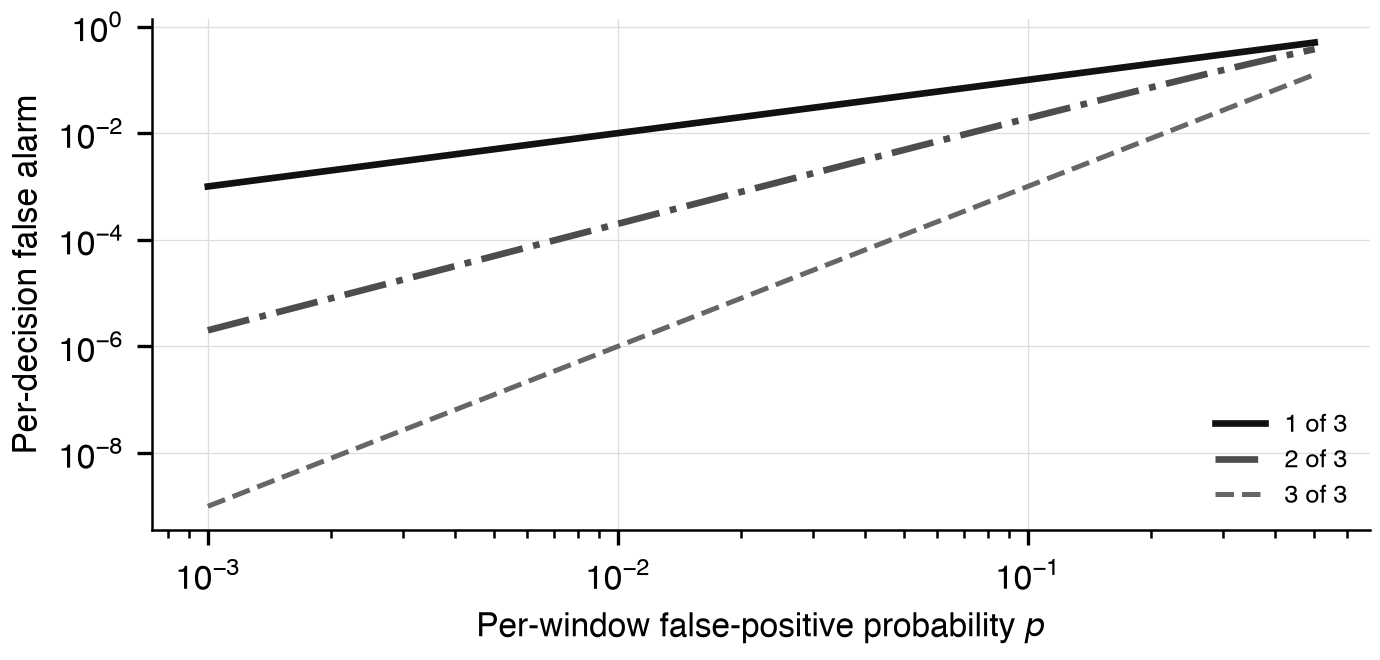
\includegraphics[width=0.7\textwidth]{kofn.png}
\caption{Analytical per-decision false-alarm probability of the $k$-of-3 rule, assuming independent windows}
\label{fig:kofn}
\end{figure}

\subsection{Tuning Against a False-Alarm Budget}
Instead of a fixed threshold, every validation clip is replayed through the exact alert rule, one class at a time, and for every candidate $(\theta_c,k_c)$ (thresholds 0.05--0.999, $k_c\in\{1,2,3\}$) the detection rate $D_c$ (share of the class's clips that raise its alert) and false-alarm rate $A_c$ (alerts per hour on validation audio without the class, including other classes' clips) are measured. The settings solve
\begin{equation}
\max_{\{\theta_c,k_c\}}\ \sum_c w_c\,D_c(\theta_c,k_c)\quad\text{subject to}\quad\sum_c A_c(\theta_c,k_c)\le B,
\end{equation}
found with a Lagrangian sweep. We chose $B=4$ per hour (Fig.~\ref{fig:budget}); solving the same problem at $B\in\{1,2,4,8,16\}$ gives the application's five-step sensitivity setting.

\begin{figure}[h]
\centering
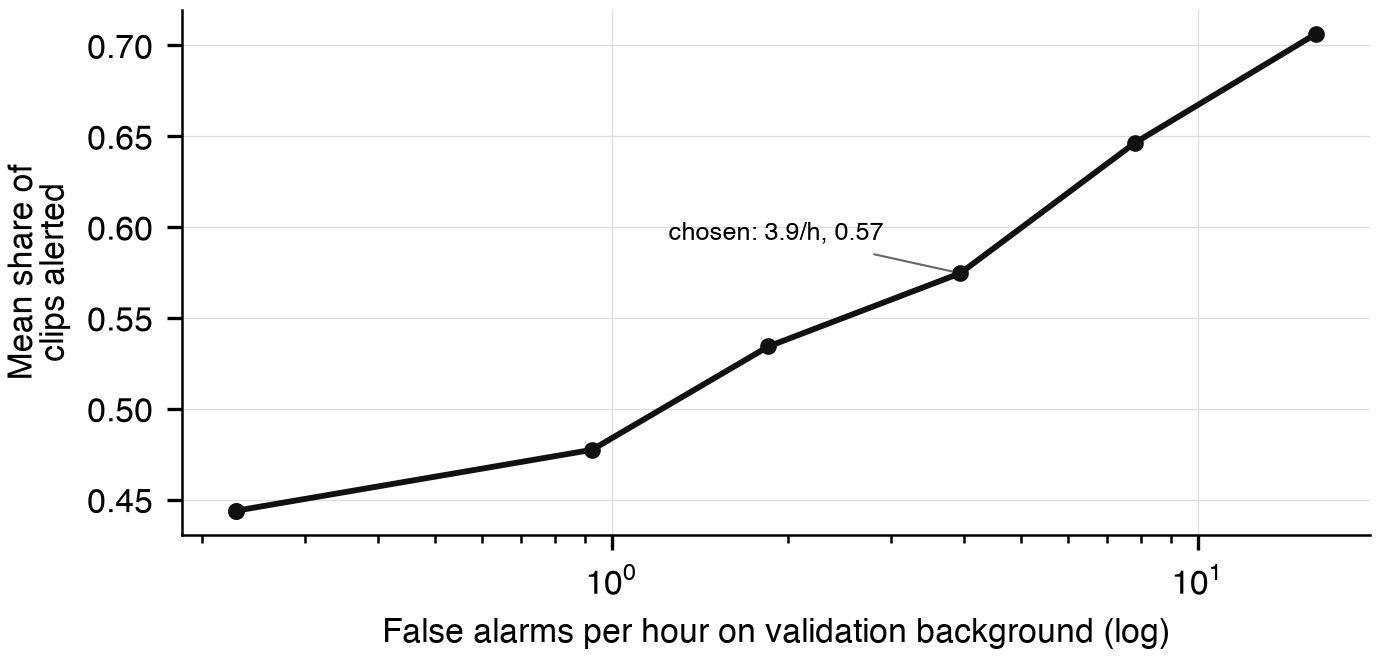
\includegraphics[width=0.75\textwidth]{budget.png}
\caption{Mean share of validation clips alerted against the false-alarm budget (same model)}
\label{fig:budget}
\end{figure}

\subsection{Home Calibration}
The user records a sound three times where it happens. For each recording the application computes the highest threshold at which the deployed rule would still alert on it, and sets that class's threshold 0.5 log-odds below the weakest recording, but never below its threshold in the most permissive tuned sensitivity step (16 false alarms per hour) and never above the current one. An optional recording of ordinary home sound raises the threshold again if that sound would fire. Only the threshold is stored. The same mathematics is implemented in Python and Kotlin and unit-tested in both.

\section{Tools and Standards}
The pipeline uses Python 3.11, TensorFlow 2.16 and TensorFlow Lite, NumPy and scikit-learn; the application uses Flutter 3.47, Kotlin 2.4 and TensorFlow Lite 2.16 on Android (API 26+); the firmware uses PlatformIO with the ESP32 Arduino core. The wristband link follows the Bluetooth Low Energy GATT model of the Bluetooth Core Specification (whose radio derives from IEEE 802.15.1), model scores use IEEE 754 single-precision floating point, the smoke-alarm vibration follows the ISO 8201 temporal-three pattern \cite{iso8201}, and software verification follows the unit- and integration-testing practices of IEEE 829/ISO/IEC/IEEE 29119 (44 Python, 50 Android and 19 Flutter tests).

\textit{Summary:} SAHARA combines a frozen pretrained embedding, a small cost-weighted head, an alert rule tuned against a false-alarm budget, a speech path for name calls and a privacy-preserving Android implementation, with a wristband designed around the same protocol.

% ================================================================ Chapter 4
\chapter{Results and Analysis}
This chapter reports detection on held-out public data, the effect of alert tuning, results under Indian conditions, home calibration, name calls and on-device cost. Model selection and alert tuning used only the validation split; the test split was used once.

\section{Detection on Held-Out Public Data}
The selected model reaches 0.778 mAP and a macro F1 of 0.670 on the public test set (Table~\ref{tab:perclass}, Fig.~\ref{fig:ap}). Played as a continuous stream through the deployed rule, it raises 3.5 false alarms per hour on 3.4 hours of public test background, mostly ``siren''. The safety classes are strongest: 22 of 27 smoke-alarm and 28 of 34 siren clips raise an alert. Glass break has high AP (0.827) but alerts on 56 of 97 clips because the budget forced a threshold of 0.93. Knocking (0.604) and appliance beep (0.567) are weakest; their brief, varied sounds limit the model rather than the rule. On synthetic mixtures at $-5$ to 10\,dB, mAP falls to 0.666 and clip detection drops sharply for doorbell (7 of 57), knocking (3 of 100) and appliance beep (9 of 101), showing that loud background remains the main challenge. Fig.~\ref{fig:conf} shows the confusion matrix.

\begin{table}[h]
\caption{Public test set per class at the deployed rule}
\label{tab:perclass}
\centering\small
\begin{tabular}{@{}lrrrrrrr@{}}
\toprule
Class & $\theta_c$ & $k_c$ & AP & Precision & Recall & F1 & Clips alerted\\
\midrule
Smoke alarm$^\dagger$ & 0.81 & 2 & 0.916 & 0.882 & 0.836 & 0.858 & 22/27\\
Doorbell & 0.995 & 1 & 0.711 & 1.000 & 0.276 & 0.432 & 13/35\\
Siren$^\dagger$ & 0.91 & 1 & 0.875 & 0.830 & 0.804 & 0.817 & 28/34\\
Knocking & 0.95 & 1 & 0.604 & 0.976 & 0.260 & 0.410 & 21/73\\
Dog bark & 0.98 & 1 & 0.908 & 0.994 & 0.737 & 0.847 & 67/90\\
Baby cry & 0.99 & 2 & 0.817 & 0.955 & 0.568 & 0.712 & 17/25\\
Glass break$^\dagger$ & 0.93 & 1 & 0.827 & 0.919 & 0.693 & 0.790 & 56/97\\
Appliance beep & 0.90 & 3 & 0.567 & 0.910 & 0.341 & 0.496 & 17/78\\
\midrule
Mean & & & 0.778 & & & 0.670 & 0.56\\
\bottomrule
\end{tabular}
\end{table}

\begin{figure}[h]
\centering
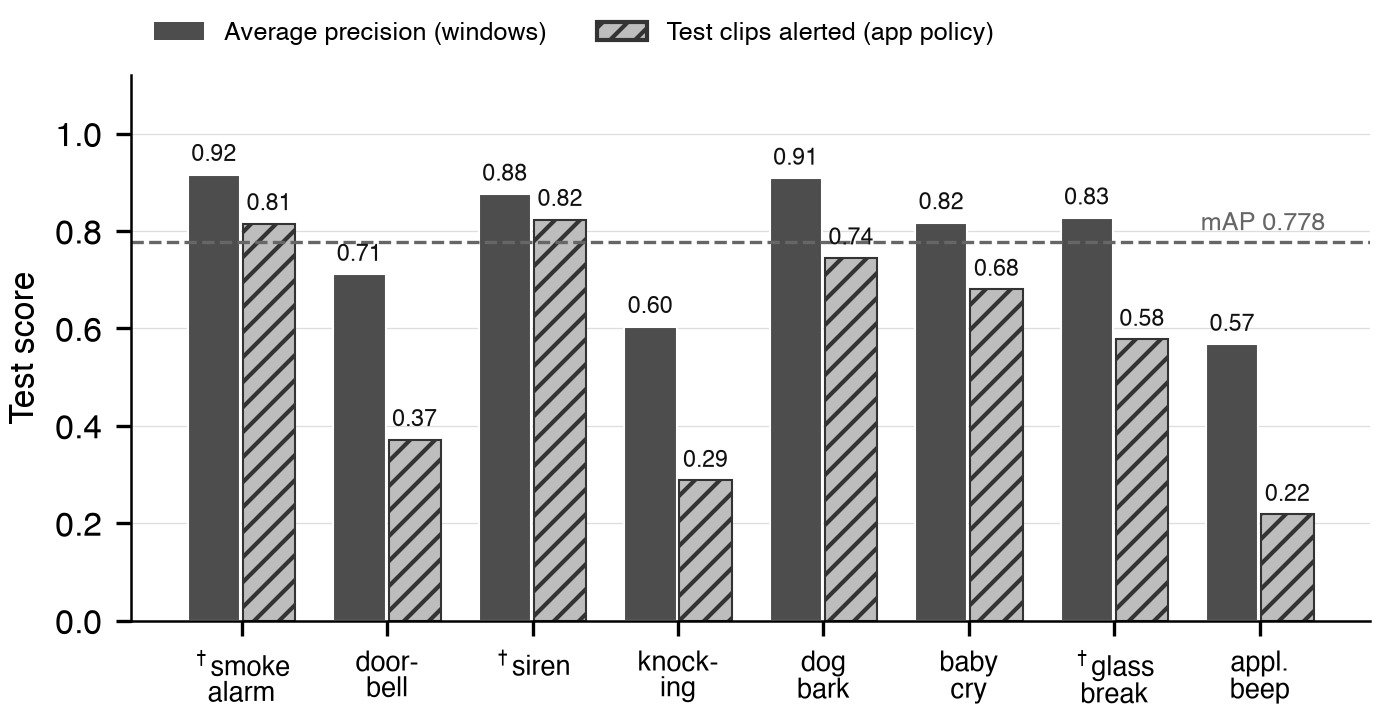
\includegraphics[width=0.8\textwidth]{test_ap.png}
\caption{Per-class test AP and share of test clips alerted under the deployed rule (public test set)}
\label{fig:ap}
\end{figure}

\begin{figure}[h]
\centering
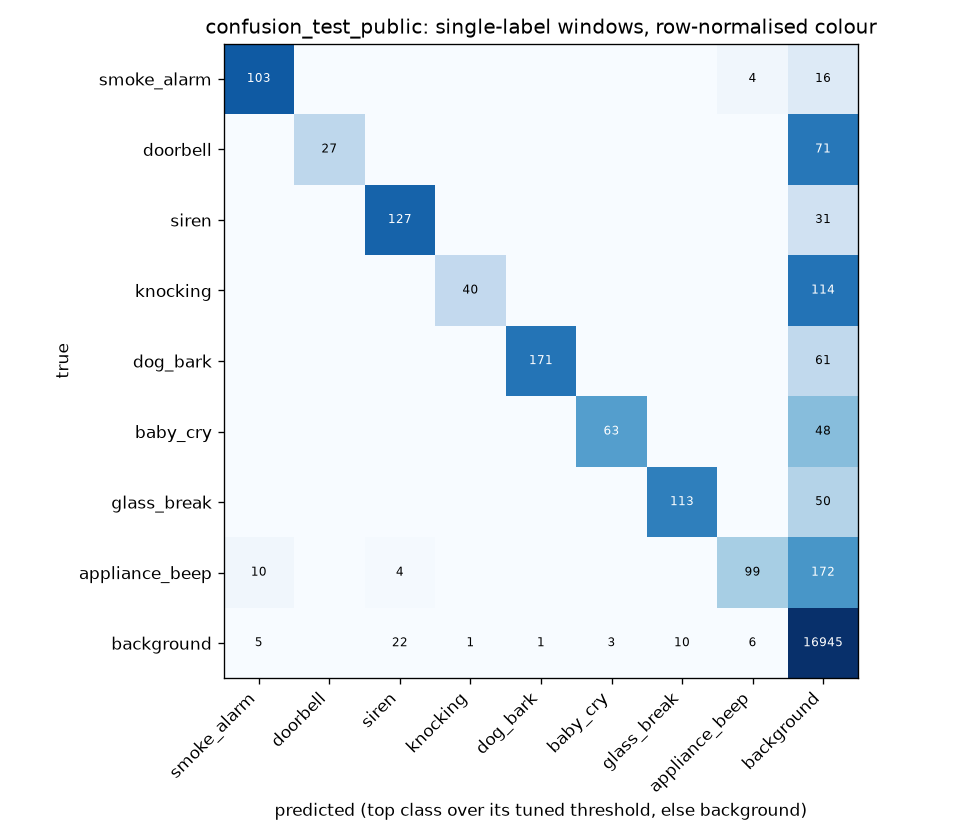
\includegraphics[width=0.6\textwidth]{confusion_test_public.png}
\caption{Confusion matrix of alerts on the public test set}
\label{fig:conf}
\end{figure}

\section{What the Alert Tuning Buys}
Table~\ref{tab:ablation} replays all 2,435 real test clips (4.6 hours) through three rules on the same model. False alarms here count alerts for a class on any audio without it, including other classes' clips, so they are higher than the background-only figure above. The fixed design of a 0.5 threshold with 2-of-3 smoothing (one window for safety classes) produces 34.1 false alarms per hour, more than one every two minutes, which no user would tolerate. Budget tuning brings this to 6.1 per hour while still alerting on 54\,\% of clips and 69\,\% of safety-class clips. Table~\ref{tab:sens} shows that the five sensitivity steps keep the expected trade-off on unseen test audio.

\begin{table}[h]
\caption{Same model, three alert rules, on all real test audio}
\label{tab:ablation}
\centering\small
\begin{tabular}{@{}lrrr@{}}
\toprule
Alert rule & Clips alerted & Safety clips & False alarms/h\\
\midrule
$\theta=0.5$, 1 window & 0.766 & 0.838 & 49.1\\
$\theta=0.5$, 1 (safety) or 2 of 3 windows & 0.688 & 0.838 & 34.1\\
Tuned $(\theta_c,k_c)$, 4/h budget (SAHARA) & 0.538 & 0.692 & 6.1\\
\bottomrule
\end{tabular}
\end{table}

\begin{table}[h]
\caption{Sensitivity steps measured on all real test audio}
\label{tab:sens}
\centering\small
\begin{tabular}{@{}lrrr@{}}
\toprule
Step (tuned budget) & Clips alerted & Safety clips & False alarms/h\\
\midrule
Fewest alerts (1/h) & 0.466 & 0.589 & 2.5\\
Fewer alerts (2/h) & 0.502 & 0.605 & 3.4\\
Balanced, default (4/h) & 0.538 & 0.692 & 6.1\\
More alerts (8/h) & 0.613 & 0.716 & 13.1\\
Most alerts (16/h) & 0.669 & 0.719 & 20.6\\
\bottomrule
\end{tabular}
\end{table}

\section{Indian Conditions}
In five-fold cross-validation over all 329 SAHARA-IN clips with random folds, adding them to training (weighted ten times) raises mAP from 0.621 to 0.822 and the clips that raise an alert from 45 to 100 of 269 (Table~\ref{tab:cv}). The gains are largest where Indian sources differ most from public data: smoke alarm AP rises from 0.385 to 0.801, knocking from 0.482 to 0.763, doorbell (melodic Indian chimes) from 0.521 to 0.824 and glass break from 0.208 to 0.476.

These folds, however, place other clips of the same sitting (the same phone, room and often the same doorbell) in training. Holding out whole recording sessions instead, the team data no longer raises mAP (0.621 without, 0.600 with; Fig.~\ref{fig:indian}). It still helps doorbells (0.521 to 0.691) and catches more baby cries (2 to 5 of 14) and beeps (9 to 12 of 59) in unseen homes, but knocking and glass break, each dominated by one session, get worse. The field recordings therefore teach the model a particular home's sounds far better than Indian sounds in general. On the held-out test split, which shares sessions with training, the model reaches 0.831 mAP and alerts on 37 of 105 Indian clips (a model trained before the latest upload: 0.698 and 31); we read this as performance in homes the model has heard.

\begin{table}[h]
\caption{SAHARA-IN five-fold cross-validation, AP without and with team data}
\label{tab:cv}
\centering\small
\begin{tabular}{@{}lrrrr@{}}
\toprule
 & \multicolumn{2}{c}{Random folds} & \multicolumn{2}{c}{Sessions held out}\\
Class & without & with & without & with\\
\midrule
Smoke alarm & 0.385 & 0.801 & 0.385 & 0.405\\
Doorbell & 0.521 & 0.824 & 0.521 & 0.691\\
Siren & 0.657 & 0.917 & 0.657 & 0.613\\
Knocking & 0.482 & 0.763 & 0.482 & 0.262\\
Dog bark & 0.932 & 0.932 & 0.932 & 0.932\\
Baby cry & 0.925 & 0.928 & 0.925 & 0.927\\
Glass break & 0.208 & 0.476 & 0.208 & 0.087\\
Appliance beep & 0.858 & 0.932 & 0.858 & 0.879\\
\midrule
mAP & 0.621 & 0.822 & 0.621 & 0.600\\
\bottomrule
\end{tabular}
\end{table}

\begin{figure}[h]
\centering
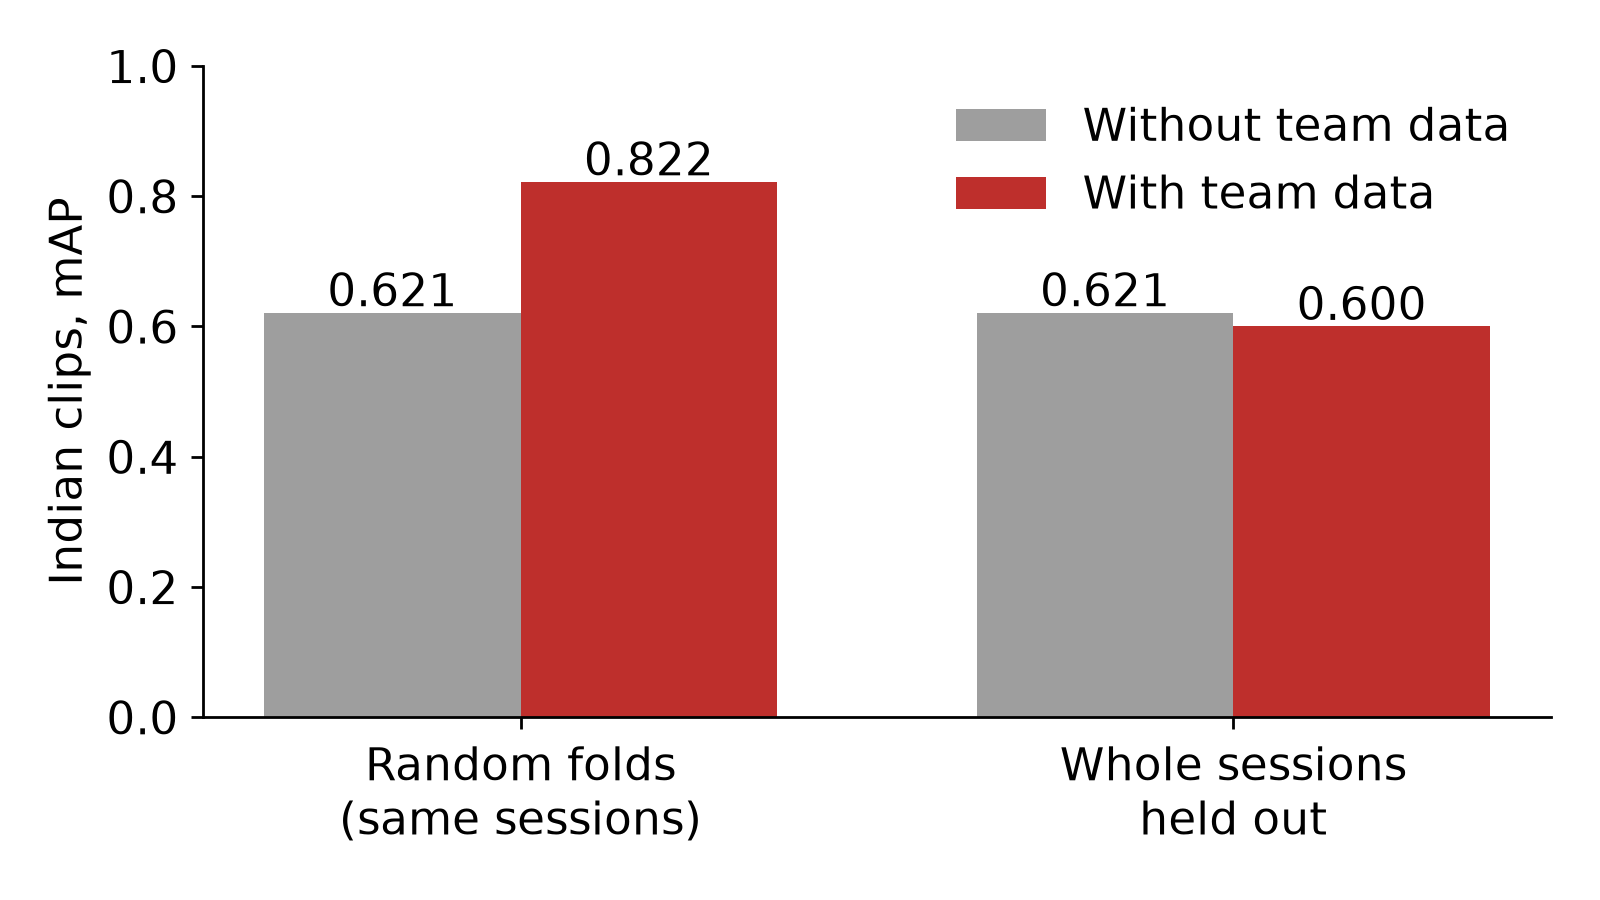
\includegraphics[width=0.65\textwidth]{indian_cv.png}
\caption{SAHARA-IN cross-validation mAP with random folds and with whole sessions held out}
\label{fig:indian}
\end{figure}

\section{Home Calibration}
Home calibration was measured on the session-held-out models: three clips of an unseen session play the calibration recordings and the rest are the events to catch, over 20 random draws. Across 17 session--class pairs, the share of events alerted rises from 19\,\% to 35\,\% (Fig.~\ref{fig:calib}), for about one extra false alarm per hour per calibrated class on the public test background. Doorbells gain most (for example 20\,\% to 83\,\%), followed by appliance beeps and baby cries; knocking, glass break and smoke alarm do not gain, because in those sessions the model's scores stay below even the most permissive tested threshold.

\begin{figure}[h]
\centering
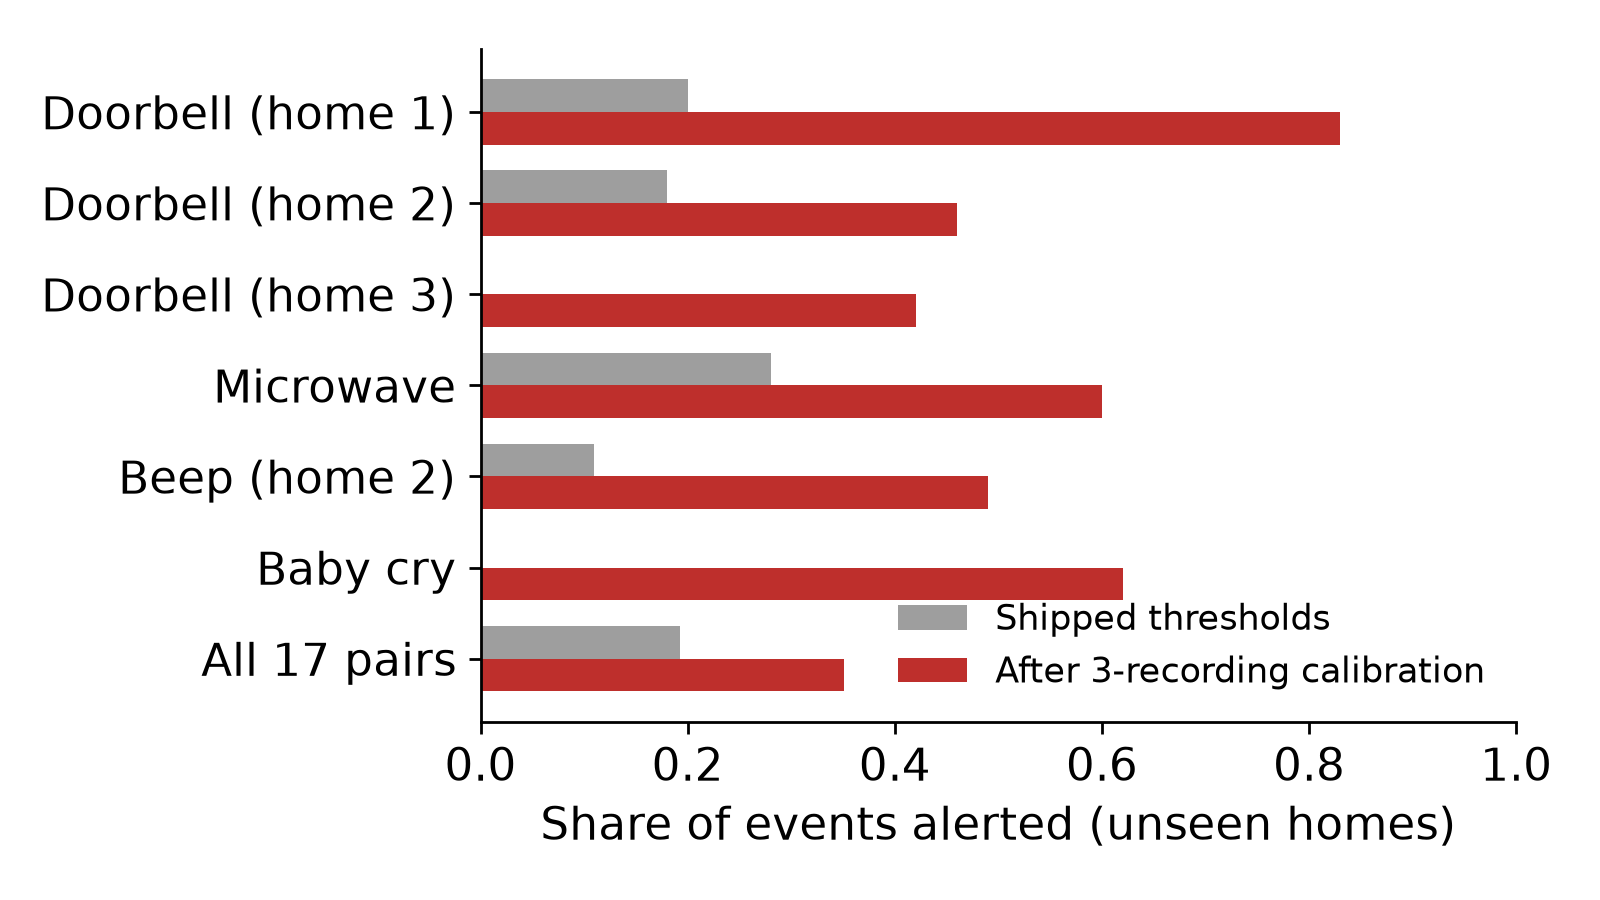
\includegraphics[width=0.7\textwidth]{calibration.png}
\caption{Share of events alerted in unseen homes before and after three-recording calibration}
\label{fig:calib}
\end{figure}

\section{Name Calls and Callers}
Table~\ref{tab:name} reports the name-call model with one recorder left out: the spotter is trained without any of that person's clips or background scenes, then scored on them, so every tested voice is new. Similar names are the hardest case. For caller identity, leaving one clip out while the rest enrol each caller names the right person in 29 of 38 calls; with a caller not enrolled, 82\,\% of their calls are reported as ``Someone''. Each team member recorded on their own phone and in their own room, so the caller figures partly measure phone and room identity and are likely optimistic.

\begin{table}[h]
\caption{Name-call detection, leave one recorder out (38 calls of ``Aryan'')}
\label{tab:name}
\centering\small
\begin{tabular}{@{}lrr@{}}
\toprule
Negatives & ROC AUC & Equal error rate\\
\midrule
Background scenes (TV, kitchen, street, temple) & 0.872 & 19\,\%\\
Similar names (Arya, Aryanshi, others; 69 clips) & 0.743 & 32\,\%\\
Both & 0.821 & 24\,\%\\
\bottomrule
\end{tabular}
\end{table}

\section{On-Device Cost}
Table~\ref{tab:device} reports the deployment on a Samsung Galaxy S24 (Android 16). The application path was verified against the evaluation pipeline: 54 test clips replayed through the application's exact code raise the same alerts in 54 of 54 cases. In a speaker test the phone alerted 1.0--2.5\,s after sound onset, within the latency bound of Section 3.5.2. Laptop-speaker playback triggered smoke-alarm and siren alerts with the screen on and off, but small speakers barely reproduce knocks, barks and doorbells, so those classes need real-source tests.

\begin{table}[h]
\caption{On-device cost (Samsung Galaxy S24, Android 16)}
\label{tab:device}
\centering\small
\begin{tabular}{@{}lr@{}}
\toprule
Measure & Value\\
\midrule
Head parameters & 296,328\\
Model files: YAMNet / head / name call & 15.0 / 1.2 / 8.1 MB\\
INT8 head size, test mAP change & 0.29 MB, $-0.015$\\
Release APK (arm64) & 45.8 MB\\
Inference per window, screen on / off & 20--29 / 47--49 ms\\
Memory (debug build, PSS) & 128.9 MB\\
Sound onset to phone alert & 1.0--2.5 s\\
Phone battery drain while listening & not yet measured\\
\bottomrule
\end{tabular}
\end{table}

\section{Discussion}
At four false alarms per hour the model alerts on about 58\,\% of validation events, and quadrupling the budget raises this only to 71\,\%, so better detection of brief sounds needs a stronger model or more data, not a looser rule. Max-pooling the two embeddings instead of averaging them, tried to stop brief sounds from being diluted, changed nothing over five seeds (validation score 0.609 against 0.614), which indicates that a brief sound is diluted inside YAMNet's 0.96\,s patch; fine-tuning YAMNet's last layers is the next step. The strongest practical lever for Indian homes is per-home adaptation, which calibration provides.

\textit{Summary:} SAHARA reaches 0.778 mAP at 3.5 false alarms per hour on public data, budget tuning cuts false alarms more than five-fold, Indian recordings help most in the homes they come from, and three-recording calibration recovers much of the gap in unseen homes.

% ================================================================ Chapter 5
\chapter{Advantages, Limitations and Applications}
This chapter summarises what SAHARA does well, where it falls short and where it can be applied.

\section{Advantages}
\begin{itemize}[itemsep=2pt]
\item \textbf{Private}: all processing on the phone; no audio stored; no Internet permission.
\item \textbf{Measured false alarms}: alerts tuned to an explicit budget, with a user-selectable, measured sensitivity.
\item \textbf{Safety first}: smoke alarm, siren and glass break weighted three times and detected best.
\item \textbf{Name calls with caller identity}, for any voice.
\item \textbf{Adapts to a home}: three-recording calibration and custom sounds.
\item \textbf{Low cost}: runs on an existing Android phone; the wristband is designed at about Rs.~870, with no smartwatch required.
\item \textbf{Distinguishable haptics}: nine class-coded vibration patterns, identical on phone and band.
\item \textbf{Open-set awareness}: quiet notices for hundreds of other sounds without false urgency.
\end{itemize}

\section{Limitations}
\begin{itemize}[itemsep=2pt]
\item Brief sounds (knocking, appliance beeps) are detected least often, and loud background lowers detection.
\item SAHARA-IN is small (20 clips per safety class) and comes from few sessions; transfer to unseen Indian homes is not yet shown without calibration.
\item The name spotter is trained for one name and confuses similar names about a third of the time; its speech models are licensed for non-commercial use only.
\item The wristband has not yet been built; its delay, current and battery life are unmeasured, as is phone battery drain over a day.
\item No study with DHH participants has been conducted yet.
\end{itemize}

\section{Applications}
\begin{itemize}[itemsep=2pt]
\item Home safety and daily-life awareness for DHH individuals and families.
\item Elderly people with age-related hearing loss living alone.
\item Assisted-living facilities, hostels and workplaces that employ DHH staff.
\item Noisy environments where hearing people also miss alarms (factories, people wearing headphones).
\item A research platform for on-device, privacy-preserving sound event detection in Indian environments.
\end{itemize}

\textit{Summary:} SAHARA's strengths are privacy, measured false alarms and adaptability; its main limitations are brief sounds, the small Indian dataset and the not-yet-built wristband.

% ================================================================ Chapter 6
\chapter{Conclusion and Future Scope}
\section{Conclusion}
This project designed, implemented and evaluated SAHARA, a real-time, fully on-device sound event detection and alert system for Deaf and Hard-of-Hearing users. A frozen YAMNet encoder with a 296k-parameter head detects eight household sounds on an Android phone, a speech path tells users when their name is called and by whom, and every alert is shown full-screen and played as a class-coded vibration. Tuning each class's threshold and temporal rule against an explicit false-alarm budget cut false alarms on the same model from 34.1 to 6.1 per hour, and the system reaches 0.778 mAP at 3.5 false alarms per hour of continuous public background. Field recordings from Mumbai homes taught the model those homes' sounds but not yet unseen ones, and a three-recording calibration step raised the share of events alerted in unseen homes from 19\,\% to 35\,\%. The system keeps no audio, needs no network and runs in 20--29\,ms per window on a current phone.

\section{Future Scope}
\begin{itemize}[itemsep=2pt]
\item Build the ESP32 wristband and measure alert delay, current draw and battery life.
\item Fine-tune YAMNet's last layers and use its finer internal time steps to improve brief sounds.
\item Record many more Indian households under a fixed protocol, with household and device metadata, to measure transfer to unseen homes.
\item Run a field study with DHH users in Mumbai, measuring missed events, alert fatigue and recognition of the vibration patterns.
\item Add classes such as pressure-cooker whistles and phone ringing, and support any user's name.
\item Measure phone battery drain over a full day and optimise the duty cycle.
\end{itemize}

% ================================================================ References
\begin{thebibliography}{99}
\addcontentsline{toc}{chapter}{References}
\bibitem{who2021} World Health Organization, \textit{World Report on Hearing}. Geneva: WHO, 2021.
\bibitem{nppcd} Directorate General of Health Services, Ministry of Health \& Family Welfare, Government of India, ``National Programme for Prevention and Control of Deafness (NPPCD).'' [Online]. Available: \url{https://dghs.mohfw.gov.in}
\bibitem{census2011} Office of the Registrar General and Census Commissioner, India, \textit{Census of India 2011: Data on Disability}. New Delhi, 2011.
\bibitem{gemmeke2017} J. F. Gemmeke, D. P. W. Ellis, D. Freedman, A. Jansen, W. Lawrence, R. C. Moore, M. Plakal, and M. Ritter, ``Audio Set: An ontology and human-labeled dataset for audio events,'' in \textit{Proc. IEEE ICASSP}, 2017, pp. 776--780.
\bibitem{fonseca2022} E. Fonseca, X. Favory, J. Pons, F. Font, and X. Serra, ``FSD50K: An open dataset of human-labeled sound events,'' \textit{IEEE/ACM Trans. Audio, Speech, Lang. Process.}, vol. 30, pp. 829--852, 2022.
\bibitem{hershey2017} S. Hershey \textit{et al.}, ``CNN architectures for large-scale audio classification,'' in \textit{Proc. IEEE ICASSP}, 2017, pp. 131--135.
\bibitem{kong2020} Q. Kong, Y. Cao, T. Iqbal, Y. Wang, W. Wang, and M. D. Plumbley, ``PANNs: Large-scale pretrained audio neural networks for audio pattern recognition,'' \textit{IEEE/ACM Trans. Audio, Speech, Lang. Process.}, vol. 28, pp. 2880--2894, 2020.
\bibitem{yamnet} M. Plakal and D. Ellis, ``YAMNet,'' TensorFlow Model Garden, 2020. [Online]. Available: \url{https://github.com/tensorflow/models/tree/master/research/audioset/yamnet}
\bibitem{howard2017} A. G. Howard \textit{et al.}, ``MobileNets: Efficient convolutional neural networks for mobile vision applications,'' arXiv:1704.04861, 2017.
\bibitem{bragg2016} D. Bragg, N. Huynh, and R. E. Ladner, ``A personalizable mobile sound detector app design for deaf and hard-of-hearing users,'' in \textit{Proc. ACM ASSETS}, 2016, pp. 3--13.
\bibitem{jain2020homesound} D. Jain \textit{et al.}, ``HomeSound: An iterative field deployment of an in-home sound awareness system for deaf or hard of hearing users,'' in \textit{Proc. CHI Conf. Human Factors in Computing Systems}, 2020.
\bibitem{jain2020soundwatch} D. Jain, H. Ngo, P. Patel, S. Goodman, L. Findlater, and J. Froehlich, ``SoundWatch: Exploring smartwatch-based deep learning approaches to support sound awareness for deaf and hard of hearing users,'' in \textit{Proc. ACM ASSETS}, 2020.
\bibitem{jain2022protosound} D. Jain \textit{et al.}, ``ProtoSound: A personalized and scalable sound recognition system for deaf and hard-of-hearing users,'' in \textit{Proc. CHI Conf. Human Factors in Computing Systems}, 2022.
\bibitem{huang2023} J. Z. Huang, H. Chhabria, and D. Jain, ```Not there yet': Feasibility and challenges of mobile sound recognition to support deaf and hard-of-hearing people,'' in \textit{Proc. ACM ASSETS}, 2023, pp. 1--14.
\bibitem{mesaros2021} A. Mesaros, T. Heittola, T. Virtanen, and M. D. Plumbley, ``Sound event detection: A tutorial,'' \textit{IEEE Signal Process. Mag.}, vol. 38, no. 5, pp. 67--83, 2021.
\bibitem{piczak2015} K. J. Piczak, ``ESC: Dataset for environmental sound classification,'' in \textit{Proc. ACM Multimedia}, 2015, pp. 1015--1018.
\bibitem{turpault2019} N. Turpault, R. Serizel, A. Parag Shah, and J. Salamon, ``Sound event detection in domestic environments with weakly labeled data and soundscape synthesis,'' in \textit{Proc. DCASE Workshop}, 2019, pp. 253--257.
\bibitem{cramer2019} J. Cramer, H.-H. Wu, J. Salamon, and J. P. Bello, ``Look, listen, and learn more: Design choices for deep audio embeddings,'' in \textit{Proc. IEEE ICASSP}, 2019, pp. 3852--3856.
\bibitem{gong2021} Y. Gong, Y.-A. Chung, and J. Glass, ``AST: Audio spectrogram transformer,'' in \textit{Proc. Interspeech}, 2021, pp. 571--575.
\bibitem{salamon2017} J. Salamon and J. P. Bello, ``Deep convolutional neural networks and data augmentation for environmental sound classification,'' \textit{IEEE Signal Process. Lett.}, vol. 24, no. 3, pp. 279--283, 2017.
\bibitem{kumar2016} A. Kumar and B. Raj, ``Audio event detection using weakly labeled data,'' in \textit{Proc. ACM Multimedia}, 2016, pp. 1038--1047.
\bibitem{mesaros2016} A. Mesaros, T. Heittola, and T. Virtanen, ``Metrics for polyphonic sound event detection,'' \textit{Applied Sciences}, vol. 6, no. 6, p. 162, 2016.
\bibitem{elkan2001} C. Elkan, ``The foundations of cost-sensitive learning,'' in \textit{Proc. IJCAI}, 2001, pp. 973--978.
\bibitem{jacob2018} B. Jacob \textit{et al.}, ``Quantization and training of neural networks for efficient integer-arithmetic-only inference,'' in \textit{Proc. IEEE CVPR}, 2018, pp. 2704--2713.
\bibitem{matthews2006} T. Matthews, J. Fong, F. W.-L. Ho-Ching, and J. Mankoff, ``Evaluating non-speech sound visualizations for the deaf,'' \textit{Behav. Inf. Technol.}, vol. 25, no. 4, pp. 333--351, 2006.
\bibitem{findlater2019} L. Findlater, B. Chinh, D. Jain, J. Froehlich, R. Kushalnagar, and A. C. Lin, ``Deaf and hard-of-hearing individuals' preferences for wearable and mobile sound awareness technologies,'' in \textit{Proc. CHI Conf. Human Factors in Computing Systems}, 2019.
\bibitem{goodman2020} S. M. Goodman, P. Kirchner, R. Guttman, D. Jain, J. Froehlich, and L. Findlater, ``Evaluating smartwatch-based sound feedback for deaf and hard-of-hearing users across contexts,'' in \textit{Proc. CHI Conf. Human Factors in Computing Systems}, 2020.
\bibitem{mielke2015} M. Mielke and R. Br\"uck, ``A pilot study about the smartwatch as assistive device for deaf people,'' in \textit{Proc. ACM ASSETS}, 2015, pp. 301--302.
\bibitem{liu2017ubiear} S. Liu, Z. Zhou, J. Du, L. Shangguan, J. Han, and X. Wang, ``UbiEar: Bringing location-independent sound awareness to the hard-of-hearing people with smartphones,'' \textit{Proc. ACM Interact. Mob. Wearable Ubiquitous Technol.}, vol. 1, no. 2, 2017.
\bibitem{laput2018} G. Laput, K. Ahuja, M. Goel, and C. Harrison, ``Ubicoustics: Plug-and-play acoustic activity recognition,'' in \textit{Proc. ACM UIST}, 2018.
\bibitem{snell2017} J. Snell, K. Swersky, and R. Zemel, ``Prototypical networks for few-shot learning,'' in \textit{Proc. NeurIPS}, vol. 30, 2017.
\bibitem{goodman2021} S. M. Goodman \textit{et al.}, ``Toward user-driven sound recognizer personalization with people who are d/Deaf or hard of hearing,'' \textit{Proc. ACM Interact. Mob. Wearable Ubiquitous Technol.}, vol. 5, no. 2, 2021.
\bibitem{lin2020} J. Lin, K. Kilgour, D. Roblek, and M. Sharifi, ``Training keyword spotters with limited and synthesized speech data,'' in \textit{Proc. IEEE ICASSP}, 2020, pp. 7474--7478.
\bibitem{openwakeword} D. Scripka, ``openWakeWord,'' GitHub, 2023. [Online]. Available: \url{https://github.com/dscripka/openWakeWord}
\bibitem{wan2018} L. Wan, Q. Wang, A. Papir, and I. Lopez Moreno, ``Generalized end-to-end loss for speaker verification,'' in \textit{Proc. IEEE ICASSP}, 2018, pp. 4879--4883.
\bibitem{iso8201} ISO 8201:2017, \textit{Alarm systems---Audible emergency evacuation signal---Requirements}. Geneva: ISO, 2017.
\end{thebibliography}

% ================================================================ Appendices
\clearpage
\renewcommand{\thefigure}{A.\arabic{figure}}\setcounter{figure}{0}
\chapter*{Appendix A: Soft Code Flowcharts}
\addcontentsline{toc}{chapter}{Appendix A: Soft Code Flowcharts}
\begin{figure}[h]
\centering
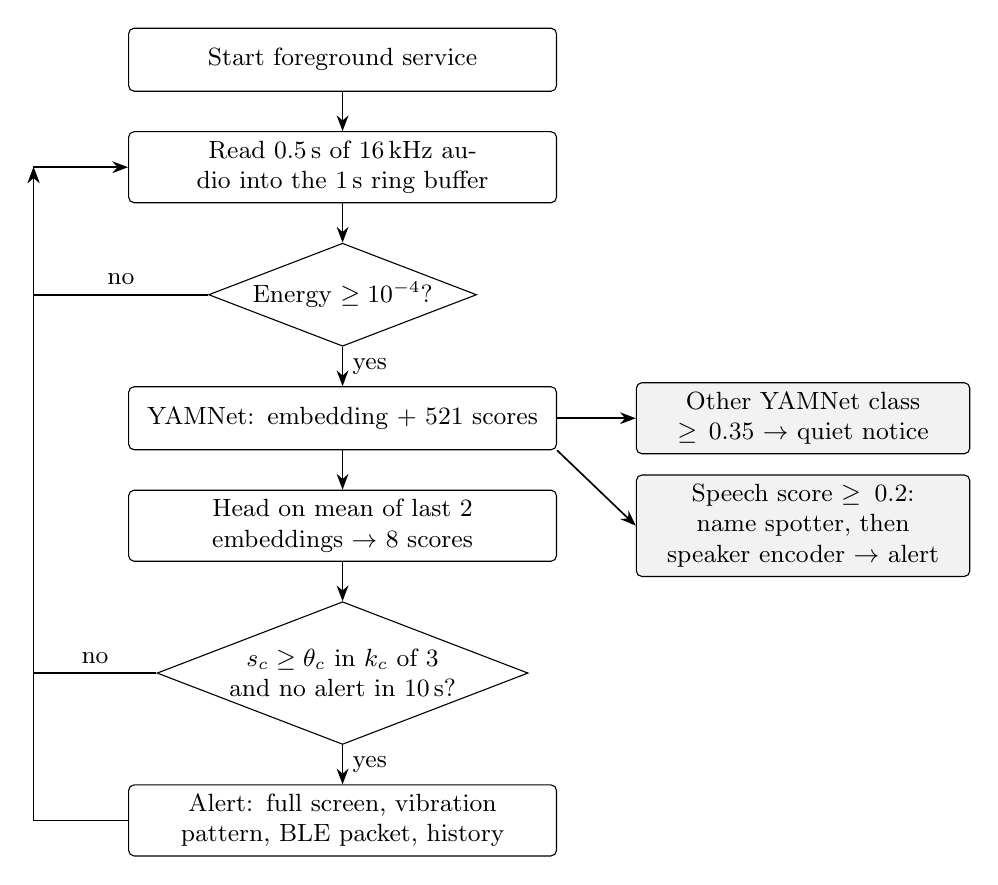
\begin{tikzpicture}[node distance=5mm and 10mm,
  b/.style={draw, rounded corners=2pt, align=center, font=\small, text width=52mm, minimum height=8mm},
  s/.style={draw, rounded corners=2pt, align=center, font=\small, text width=40mm, minimum height=8mm, fill=black!5},
  d/.style={draw, diamond, aspect=2.6, align=center, font=\small, inner sep=1pt},
  a/.style={-{Stealth[length=2mm]}, semithick}]
\node[b] (s) {Start foreground service};
\node[b, below=of s] (r) {Read 0.5\,s of 16\,kHz audio into the 1\,s ring buffer};
\node[d, below=of r] (v) {Energy $\ge 10^{-4}$?};
\node[b, below=of v] (y) {YAMNet: embedding + 521 scores};
\node[b, below=of y] (h) {Head on mean of last 2 embeddings $\rightarrow$ 8 scores};
\node[d, below=of h] (p) {$s_c\ge\theta_c$ in $k_c$ of 3\\and no alert in 10\,s?};
\node[b, below=of p] (al) {Alert: full screen, vibration pattern, BLE packet, history};
\node[s, right=of h] (sp) {Speech score $\ge 0.2$: name spotter, then speaker encoder $\rightarrow$ alert};
\node[s, right=of y] (os) {Other YAMNet class $\ge 0.35$ $\rightarrow$ quiet notice};
\draw[a] (s) -- (r); \draw[a] (r) -- (v); \draw[a] (v) -- node[right, font=\small]{yes} (y);
\draw[a] (y) -- (h); \draw[a] (h) -- (p); \draw[a] (p) -- node[right, font=\small]{yes} (al);
\draw[a] (y.east) -- (os.west); \draw[a] (y.south east) -- (sp.west);
\coordinate (L) at ([xshift=-12mm]r.west);
\draw[a] (v.west) -- node[above, font=\small]{no} (v.west -| L) -- (L) -- (r.west);
\draw[a] (p.west) -- node[above, font=\small]{no} (p.west -| L) -- (L);
\draw[a] (al.west) -- (al.west -| L) -- (L);
\end{tikzpicture}
\caption{Runtime flowchart of the on-device detection loop}
\label{fig:flow1}
\end{figure}

\begin{figure}[h]
\centering
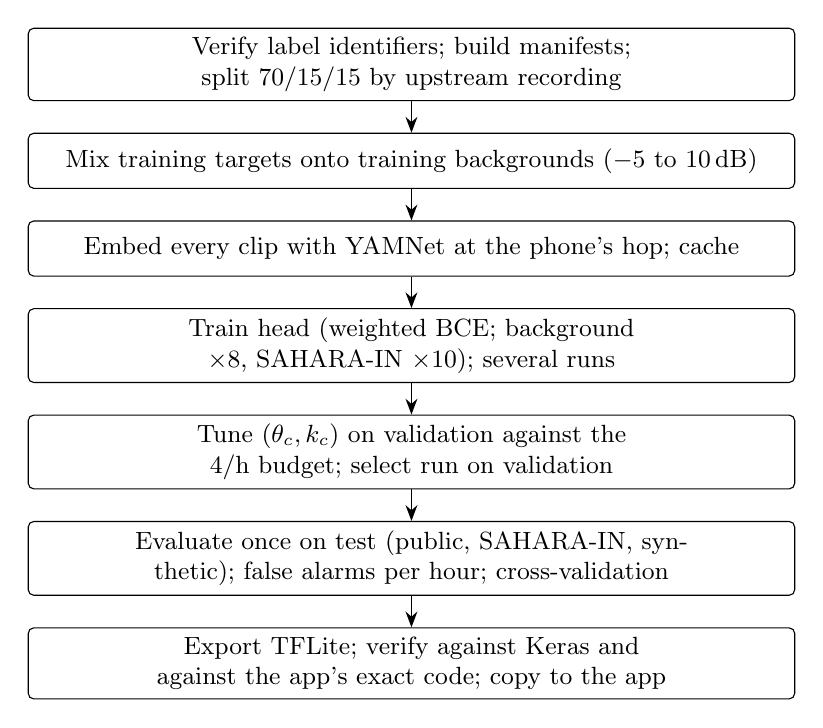
\begin{tikzpicture}[node distance=4mm,
  b/.style={draw, rounded corners=2pt, align=center, font=\small, text width=95mm, minimum height=7mm},
  a/.style={-{Stealth[length=2mm]}, semithick}]
\node[b] (1) {Verify label identifiers; build manifests; split 70/15/15 by upstream recording};
\node[b, below=of 1] (2) {Mix training targets onto training backgrounds ($-5$ to 10\,dB)};
\node[b, below=of 2] (3) {Embed every clip with YAMNet at the phone's hop; cache};
\node[b, below=of 3] (4) {Train head (weighted BCE; background $\times8$, SAHARA-IN $\times10$); several runs};
\node[b, below=of 4] (5) {Tune $(\theta_c,k_c)$ on validation against the 4/h budget; select run on validation};
\node[b, below=of 5] (6) {Evaluate once on test (public, SAHARA-IN, synthetic); false alarms per hour; cross-validation};
\node[b, below=of 6] (7) {Export TFLite; verify against Keras and against the app's exact code; copy to the app};
\foreach \i/\j in {1/2,2/3,3/4,4/5,5/6,6/7} \draw[a] (\i) -- (\j);
\end{tikzpicture}
\caption{Training and export pipeline}
\label{fig:flow2}
\end{figure}

\clearpage
\renewcommand{\thetable}{B.\arabic{table}}\setcounter{table}{0}
\chapter*{Appendix B: Data Sheets}
\addcontentsline{toc}{chapter}{Appendix B: Data Sheets}
\begin{table}[h]
\caption{Key specifications of the main wristband components (from manufacturer data sheets)}
\label{tab:datasheet}
\centering\small
\begin{tabularx}{\textwidth}{@{}lX@{}}
\toprule
Component & Key specifications\\
\midrule
ESP32-WROOM-32 & Dual-core Xtensa LX6 up to 240\,MHz; 520\,KB SRAM; 4\,MB flash; Wi-Fi 802.11 b/g/n; Bluetooth v4.2 BR/EDR and BLE; 3.0--3.6\,V supply\\
TP4056 module & 1\,A linear Li-ion charger, 4.2\,V charge termination; with DW01A + 8205A protection (over-discharge, over-current)\\
AO3400 & N-channel logic-level MOSFET, 30\,V, about 5.7\,A, low on-resistance at 2.5--4.5\,V gate drive\\
Coin motor (1027) & 10\,mm eccentric rotating mass, 3\,V rated, roughly 60--80\,mA running current\\
LDO (AP2112K-3.3 / ME6211) & 3.3\,V output, $\ge$500\,mA, low dropout for a single Li-ion cell\\
LiPo cell (502540) & 3.7\,V nominal, 500\,mAh\\
\bottomrule
\end{tabularx}
\end{table}

\begin{table}[h]
\caption{Software components}
\label{tab:software}
\centering\small
\begin{tabularx}{\textwidth}{@{}lX@{}}
\toprule
Component & Version and role\\
\midrule
Python, TensorFlow & 3.11, 2.16: training, evaluation and export\\
TensorFlow Lite & 2.16: on-device YAMNet, head and name-call models\\
YAMNet & TensorFlow Hub model (AudioSet, 521 classes, 1,024-d embeddings)\\
Flutter, Kotlin & 3.47, 2.4: user interface; native audio service and inference\\
Android & API 26 (8.0) and above; tested on Android 16\\
PlatformIO, ESP32 Arduino core & wristband firmware\\
\bottomrule
\end{tabularx}
\end{table}

\clearpage
\renewcommand{\thetable}{C.\arabic{table}}\setcounter{table}{0}
\chapter*{Appendix C: List of Components}
\addcontentsline{toc}{chapter}{Appendix C: List of Components}
\begin{table}[h]
\caption{Wristband bill of materials (approximate Indian retail prices, 2026)}
\label{tab:bom}
\centering\small
\begin{tabular}{@{}lrr@{}}
\toprule
Component & Qty & Approx.\ price (Rs.)\\
\midrule
ESP32 DevKit V1 (ESP32-WROOM-32) & 1 & 350\\
3.7\,V LiPo cell, 500\,mAh (502540) & 1 & 180\\
TP4056 USB-C charger module with protection & 1 & 35\\
3.3\,V low-dropout regulator & 1 & 20\\
10\,mm coin vibration motor, 3\,V & 1 & 40\\
AO3400 logic-level N-MOSFET & 1 & 10\\
1N4148 diodes & 2 & 4\\
Resistors (100k $\times$3, 100\,$\Omega$, 330\,$\Omega$) & 5 & 5\\
LED and slide switch & 2 & 12\\
Perfboard, wires, headers & -- & 60\\
Velcro strap and 3D-printed enclosure & 1 & 150\\
\midrule
\textbf{Total} & & \textbf{$\approx$ 870}\\
\bottomrule
\end{tabular}
\end{table}

\clearpage
\chapter*{Appendix D: List of Papers Presented and Published}
\addcontentsline{toc}{chapter}{Appendix D: List of Papers Presented and Published}
\begin{enumerate}
\item M. Mayani, A. Mishra, P. Teotia, R. Singh, and P. Rumao, ``SAHARA: A Real-Time, On-Device Sound Event Detection and Dual-Channel Alert System for the Deaf and Hard-of-Hearing, with India-Specific Acoustic Adaptation,'' submitted to the International Conference on Emerging Innovations (ICEI 2026), submission no.\ 525. Revised version with full experimental results prepared in response to the reviewers' comments.
\end{enumerate}

\end{document}
